\subsection{Gini Index}
\textit{Gini index}\cite{ginindex} measures the inequality of a
distribution. Values of 0 and 1 stand for, respectively, the
maximum homogeneity and the maximum heterogeneity.
However, this index is a function of random values: mean and
error have to be estimated.\\
A certain number of samples is created by sampling with replacement
of the average FOUR distribution: Gini index is computed for each
one of them.
Now we have a population of Gini indexes, and we can extract
mean and error: the whole process is known as
\textit{bootstrap}\cite{bootstrap}
(see \hl{Appendix 1} for error estimation).\\
In practical terms, for every level of  memory, a simulation with
twenty news is run out: Gini index' mean and error are computed
like before.
The Gini index-memory plot shows a highly non-linear behaviour:
sigmoid and gaussian seem to better represent data.\\
In order to select the best-fit function, \textit{Chi-square} is
computed for both of them. \\
Because of asymmetric error bars, the optimization function is
slightly different from the standard one, used for weighted
interpolation: see \hl{Appendix 2} for more details.
Interpolation results are shown below:

%\begin{figure}[!h]
  %\centering
  %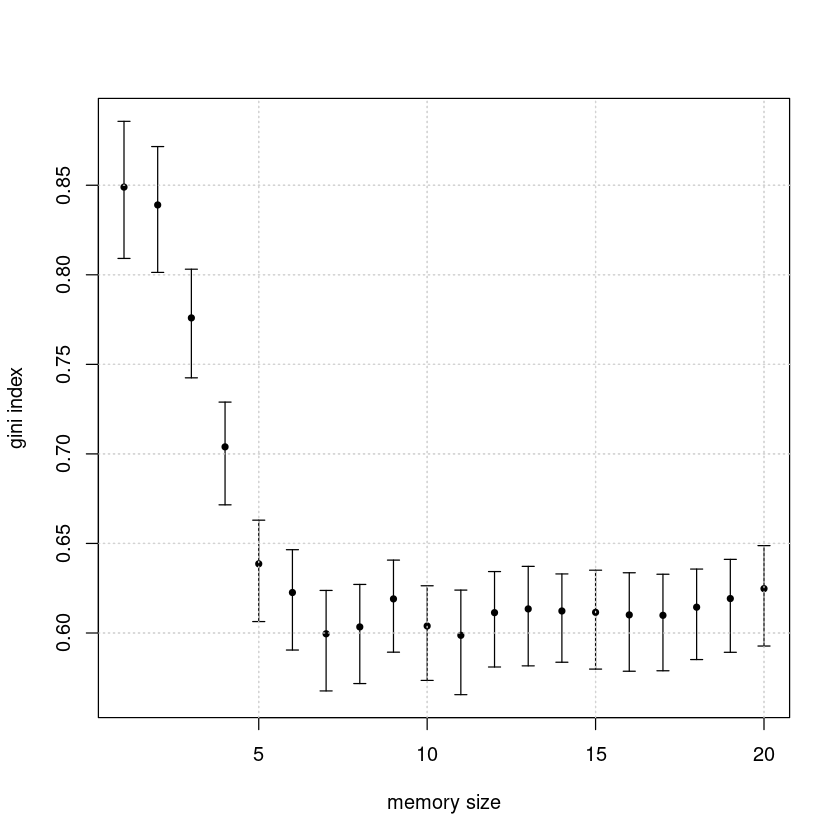
\includegraphics[width=.7\columnwidth]{img/gini_memory.png}
  %\caption{Gini index-memory plot with errorbars}
  %\label{fig:ginimem}
%\end{figure}




\begin{figure}[h]
  \centering
  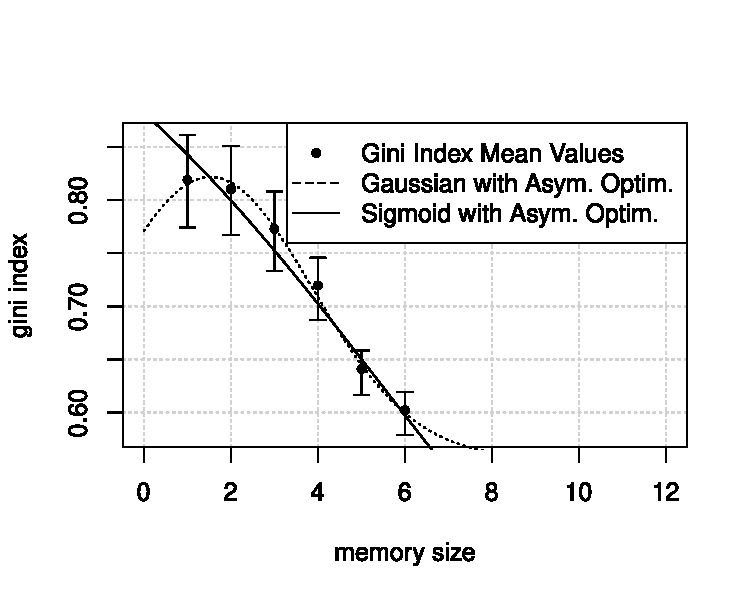
\includegraphics[trim={0cm 0cm 0cm 1cm},clip,width=.8\columnwidth]{img/gini.pdf}
  \caption{Gini index on memory size.}
  \label{fig:gini}
\end{figure}

\begin{table}[h]
  \centering
  \begin{tabular}{rSSSS}
    \toprule
    & \multicolumn{2}{c}{\textit{Gaussian Fit}} & \multicolumn{2}{c}{\textit{Sigmoid Fit}}\\
     & {$\chi^2$} & {p-value} & {$\chi^2$} & {p-value} \\ \midrule
    stde & 0.0013260 & 0.97195 & 0.00080793 & 0.97732 \\
    qant & 0.0037563 & 0.95113 & 0.0012997  & 0.97124 \\
    asym & 0.0013576 & 0.97061 & 0.00084281 & 0.97684 \\ \bottomrule
  \end{tabular}
  \caption{Reduced $\chi^2$ and respective p-value for Gaussian
    and Sigmoid fit with different non-linear optimization
    strategies.\\
    Optimization using the standard error of the Gini index
    is denoted as std, quantile bootstrap optimization\cite{quantile} as
    quant and asymmetric error bar fitting optimization as asym.}
  \label{tab:gini}
\end{table}

We can notice that, for every type of errorbar, sigmoid's
$\chi^2$ is slightly lower than gaussian one; p-value is
higher instead.
Null hypothesis, for both measures, is far from being rejected:
goodness-of-fit is solidly validated.
Hence, sigmoid is our best-fit function for gini index-memory
length plot.
